\documentclass[11pt]{article}
\usepackage{geometry}
\geometry{a4paper}
\linespread{1.1} % Line spacing

% FIGURES AND FLOATS
\usepackage{graphicx} % Required for including pictures
\usepackage{float} % Allows putting an [H] in \begin{figure} to specify the exact location of the figure
\usepackage{wrapfig} % Allows in-line images such as the example fish picture
\usepackage[font={small,it}]{caption}
\usepackage{subcaption}
\usepackage{epstopdf}
\usepackage{pifont}

% MATH
\usepackage{amssymb}
\usepackage{amsmath}
\usepackage{algorithm}
\usepackage[noend]{algpseudocode}

% OTHER
\usepackage{color}
\usepackage{xeCJK}


%%%%%%%%%%%%%%%%%%%%%%%%%%%%%%%%%%%%%%%%%%%%%%%%%%%%%%%%%%%%
\title{一周学会Linux - 韩顺平}
\author{muyi}
\begin{document}
\maketitle


\section{Linux与Unix的关系}

\subsection{Unix}
\begin{figure}[htb]
    \centering
    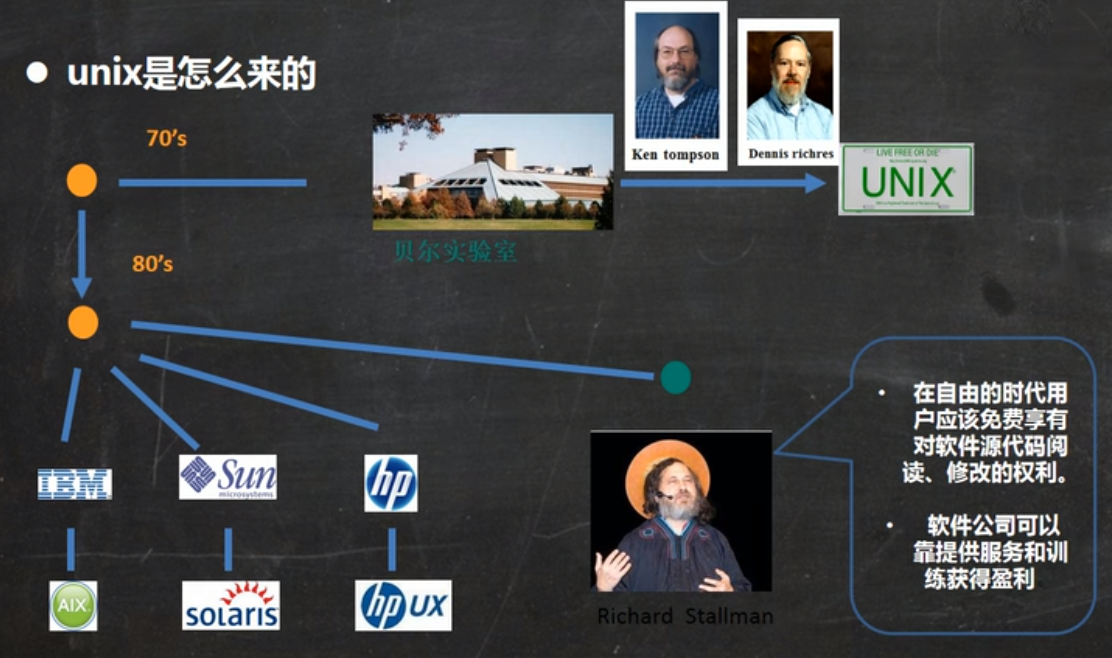
\includegraphics[scale=0.12]{imgs/unix.png}
\end{figure}

\subsection{Linux}
\begin{figure}[htb]
    \centering
    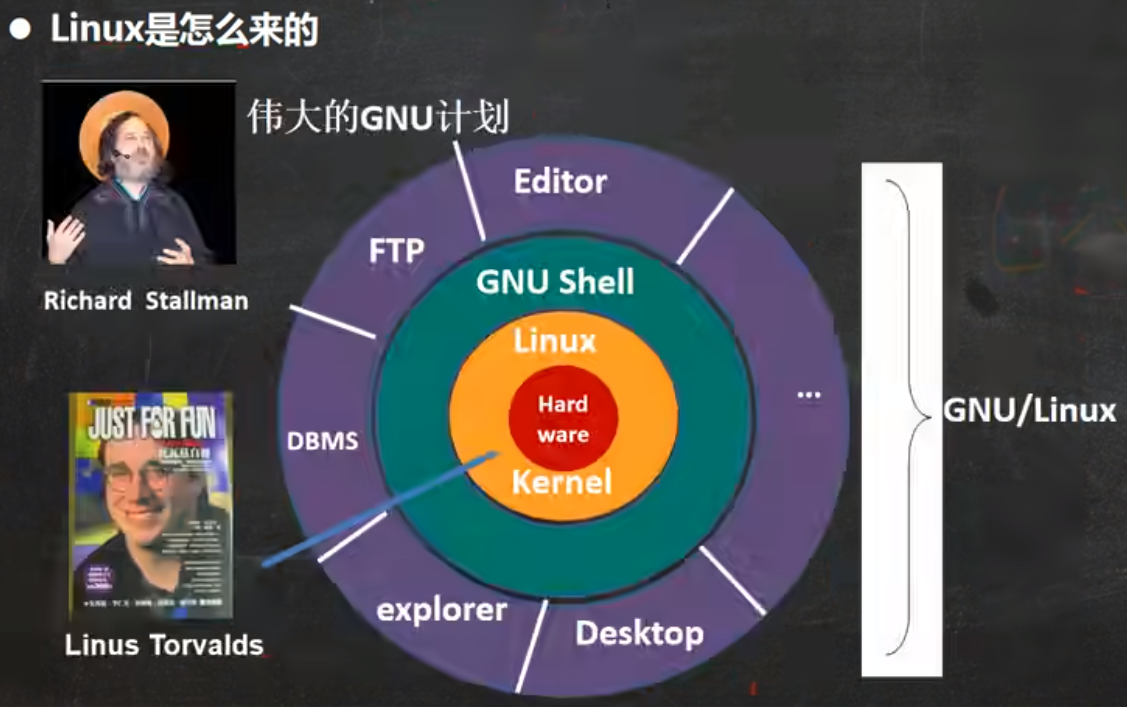
\includegraphics[scale=0.12]{imgs/gnu_linux.png}
\end{figure}

\subsection{Unix to Linux}
\begin{figure}[htb]
    \centering
    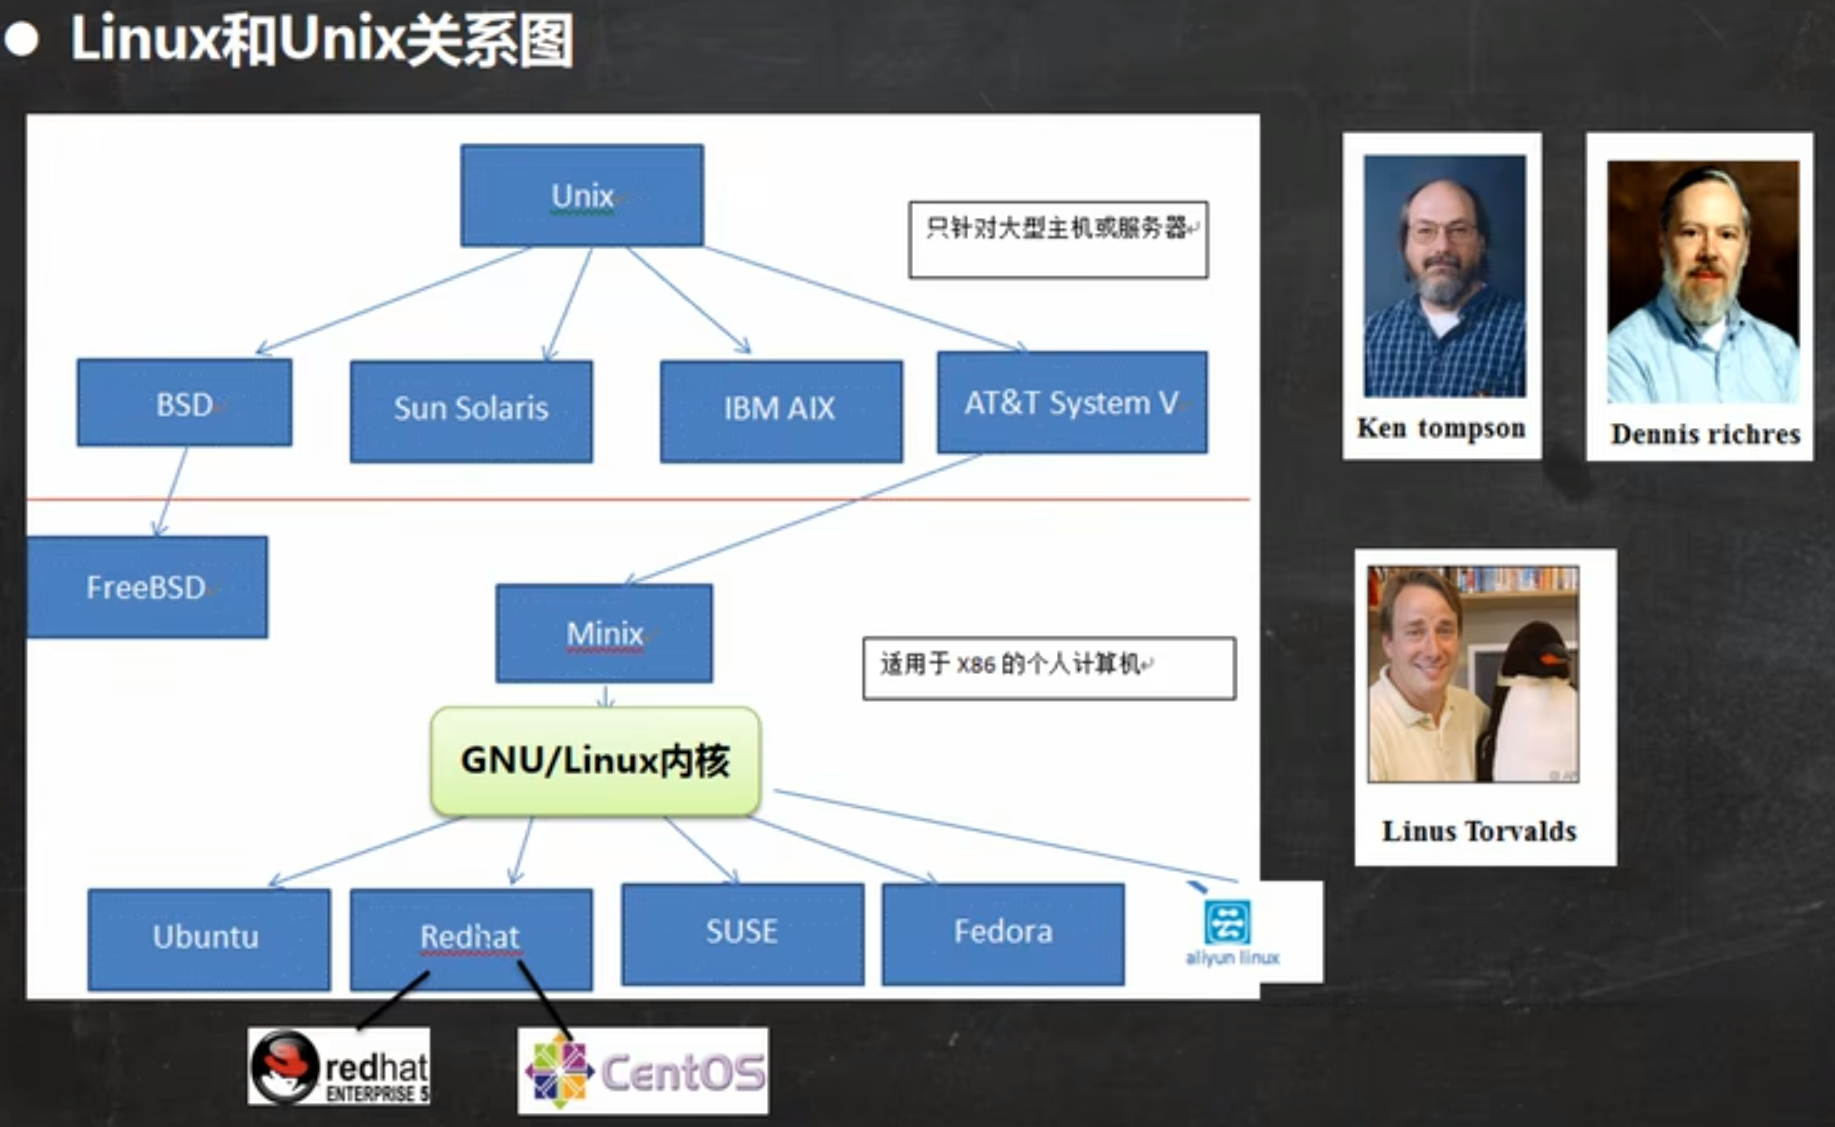
\includegraphics[scale=0.08]{imgs/unix_linux.png}
\end{figure}


\section{目录结构}
在Linux的世界里,一切皆文件。
\subsection{常见目录}
/:根目录  \\
/bin(/usr/bin, /usr/local/bin):存放常用命令  \\
/sbin(/usr/sbin, /usr/local/sbin):Super User管理员的命令  \\
/home:普通用户的主目录  \\
/root:管理员的主目录  \\
/lib:动态链接库  \\
/lost+found:当系统非法关机后这里会存放一些文件,一般为空  \\
/etc:配置文件  \\
/usr:应用程序  \\
/boot:启动文件  \\
/proc, /srv, /sys:系统相关的文件  \\
/tmp:临时文件  \\
/dev:类似设备管理器,对应硬件  \\
/media:U盘、光驱等  \\
/mnt:挂载别的文件系统  \\
/var:存放一些经常修改的内容,比如日志 \\


\section{Vim}

\subsection{三种模式}
\ding{172} 一般模式:用vim打开一个文件后就是一般模式,在此模式下可以使用复制、粘贴、删除整行等功能。  \\
\ding{173} 插入模式:在一般模式下输入i即可进入插入模式,在此模式下对文件进行编辑。  \\
\ding{174} 命令行模式:在插入模式下,先按esc键退出插入模式,然后输入:即可进入命令行模式(在一般模式下
直接输入:即可),在此模式下可以进行保存、退出、设置显示行号等操作。
\begin{figure}[htb]
    \centering
    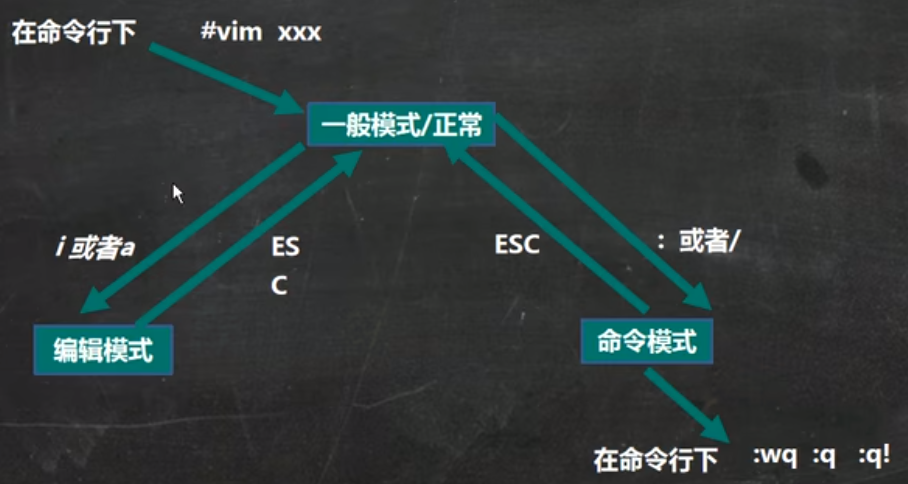
\includegraphics[scale=0.18]{imgs/vim_mode.png}
\end{figure}

\subsection{Vim快捷键}
复制当前行:yy \qquad 向下复制n行:nyy \qquad 粘贴:p \qquad 删除当前行:dd \qquad 
向下删除n行:ndd \qquad 查找关键词:/keyword \qquad 定位首行:gg \qquad 定位第n行:ngg
\qquad 定位末行:G \qquad 撤销:u

\section{关机重启}

\subsection{关机}
最常用的关机命令是shutdown,用法如下: \\
shutdown -h now \qquad 马上关机 \qquad shutdown -h 5 \qquad 5分钟后关机 \\
shutdown -r now \qquad 马上重启 \\
除了shutdown之外这几个命令也可以关机,但有细微区别:halt, poweroff, init 0.

\subsection{重启}
shutdown -r now \quad 或 \quad reboot

\subsection{同步}
sync:把内存中的数据同步到磁盘  \\
一般在关机或重启前应当先运行sync命令以防数据丢失,但目前shutdown/reboot/halt等命令在关机前均会
先调用sync命令。

\subsection{运行级别}
0:关机 \qquad 1:单用户(可在此模式下找回密码) \qquad 2:多用户,但没有网络服务 \qquad 3:
多用户,且有网络服务 \qquad 4:系统保留 \qquad 5:图形界面 \qquad 6:系统重启  \\
常用的运行级别是3和5,通过init 0/1/2/3/4/5/6指令可以切换运行级别。

\section{用户管理}
添加用户:useradd -m username(带-m参数以自动生成/home/username目录) \\
修改用户密码:passwd username \\
删除用户:userdel (-r) username(不带-r参数时删除用户但保留/home/username文件夹,带-r参数则
连同文件夹一起删除) \\
查询用户信息:id username \\
切换用户:su (-) username(若不带-仅切换用户,带-同时将当前目录切换到/home/username) \\
新增用户组:groupadd groupname \\
删除用户组:groupdel groupname \\
修改用户所属组:usermod -g groupname username(在添加用户时可以通过-g参数直接指定所属组,即
useradd -g groupname username,若没有指定组,则系统会自动新建一个和username同名的组) \\
相关文件:用户信息保存在/etc/passwd,密码信息保存在/etc/shadow,组的信息保存在/etc/group。

\section{常用指令}

\subsection{文件目录指令}

pwd:显示当前目录的绝对路径 \\
ls:显示当前目录下的文件(带-a参数显示隐藏文件,带-l参数以列表形式显示) \\
mkdir (-p) dirname:创建文件夹,带-p参数才能创建多级目录  \\
rmdir dirname:删除空目录 \qquad rm -rf dirname:删除非空目录  \\
touch filename:创建一个空文件 \\
cp (-r) source dest:拷贝文件(-r参数表示递归)  \\
mv source/oldName dest/newName:移动文件或者重命名文件  \\
cat (-n) filename:以只读方式查看文件(带-n参数显示行号)  \\
less filename:按页显示文件内容,适合用来查看较大的文件  \\
echo:输出内容到terminal,例如echo \$PATH查看环境变量 \\
tail filename:显示文件末尾10行 \qquad tail -f filename:实时监控文件内容更新 \\
$>$和$>>$:输出重定向,将本该输出到terminal的内容写入文件,例如echo 'something' > filename。
区别在于>是覆盖,$>>$是追加。  \\
ln -s source dest:创建软链接  \\
history:查看执行过的指令

\subsection{时间日期指令}
date:显示时间日期信息,也可通过添加参数格式化输出  \\
cal:显示本月日历

\subsection{搜索查找指令}
find dirname -name filename:在dirname目录下查找filename文件,输出其路径 \\
locate filename:功能和find类似,也是输出filename文件的路径,但locate指令比find指令快得多,
因为locate指令并不会真的扫描文件目录,而是在一个数据库中查找filename对应的路径。系统会每天自动
更新该数据库,所以如果用locate指令查找刚刚创建的文件会找不到,或者查找刚刚删除的文件仍显示出删除
前的路径。为避免这种情况,可以在locate前使用updatedb指令手动更新数据库。  \\
which cmdname:查看某个指令所在的路径,如which ls  \\
grep:搜索关键词,常和管道符号|一起使用,如cat filename | grep keyword

\subsection{压缩解压指令}
gzip/gunzip:gzip filename压缩文件(只能压缩为.gz),gunzip filename.gz解压文件  \\
zip/unzip:zip常用选项-r递归压缩,unzip常用选项-d指定解压文件存放目录  \\
tar:压缩用tar -zcvf filename.tar.gz files2zip,解压用tar -zxvf filename.tar.gz







    
\end{document}